\documentclass[12pt]{article}

\usepackage{geometry}
\usepackage[utf8]{inputenc}
\usepackage[polish]{babel}
\usepackage{polski}
\usepackage{hyperref}
\usepackage{graphicx}
\usepackage{verbatim}
\usepackage{acronym}
\usepackage{fancyhdr}
\usepackage[usenames]{color}

\hypersetup{
  linkbordercolor={1 1 1},
  urlbordercolor={1 1 1},
  colorlinks=false
}

\pagestyle{fancy}
\cfoot{}
\rfoot{\thepage}

\author{Michał Bugno \and Antek Piechnik}
\title{Analiza oraz wizualizacja danych meteorologicznych dla wybranych ośrodków narciarskich}
% W oparciu o bazę danych Oracle z wykorzystaniem technologii Oracle Spatial.

\begin{document}
\maketitle
\tableofcontents
\newpage

\section{Wizja projektu}
Głównym zadaniem projektu jest poznanie struktury
danych typu GIS (geographical information system), jak również analiza oraz
wykorzystanie tego typu danych w wizualizacji danych meteorologicznych. System
docelowo ma za zadanie przedstawienie sytuacji meteorologicznej na podstawie
danych zbieranych na bieżąco jak również danych historycznych zgromadzonych
poprzednio. System ma również mieć możliwość udostępniania danych/wizualizacji
historycznych na życzenie użytkownika. Do celów badania wydajności systemu
wykorzystywane będą dane z przynajmniej dwóch źródeł informacji
meteorologicznej, podczas gdy system ma domyślnie obsługiwać 4-5 stacji
narciarskich (po kilka punktów na każdą stację).

\section{Ogólna struktura systemu}

\subsection{Baza danych}
Wybraną bazą danych jest Oracle. Wyboru dokonaliśmy głównie ze względu na
możliwość dokładnego poznania tego produktu w ramach projektu jak również ze
względu na obszerne wsparcie dla danych GIS - Oracle Spatial.

\subsection{Technologia}
System jest tworzony w technologii Python Django -- posiada ona wpsarcie dla
baz Oracle (w tym Spatial) oraz jest prosta i przejrzysta zapewniając
bardziej elastyczny rozwój.

\subsection{Aplikacja pobierająca dane z internetu (crawler)}
Aplikacja będzie w rzeczywistości skryptem mającym na celu pobranie
odpowiednich danych z wcześniej przygotowanych źródeł (stron internetowych
    udostępniających informacje meteorologiczne dla konkretnych ośrodków).
Będzie on miał również możliwość aktualizowania bazy danych o pobrane
informacje, po uprzednich skonwertowaniu ich do odpowiedniego formatu.

\subsection{Renderer graficzny}
Renderer zostanie utworzony w oparciu o dane wygenerowane przez kontroler
analizy danych oraz o API systemu Google Maps który pozwoli na estetyczną
wizualizację osiągniętych wyników analizy.

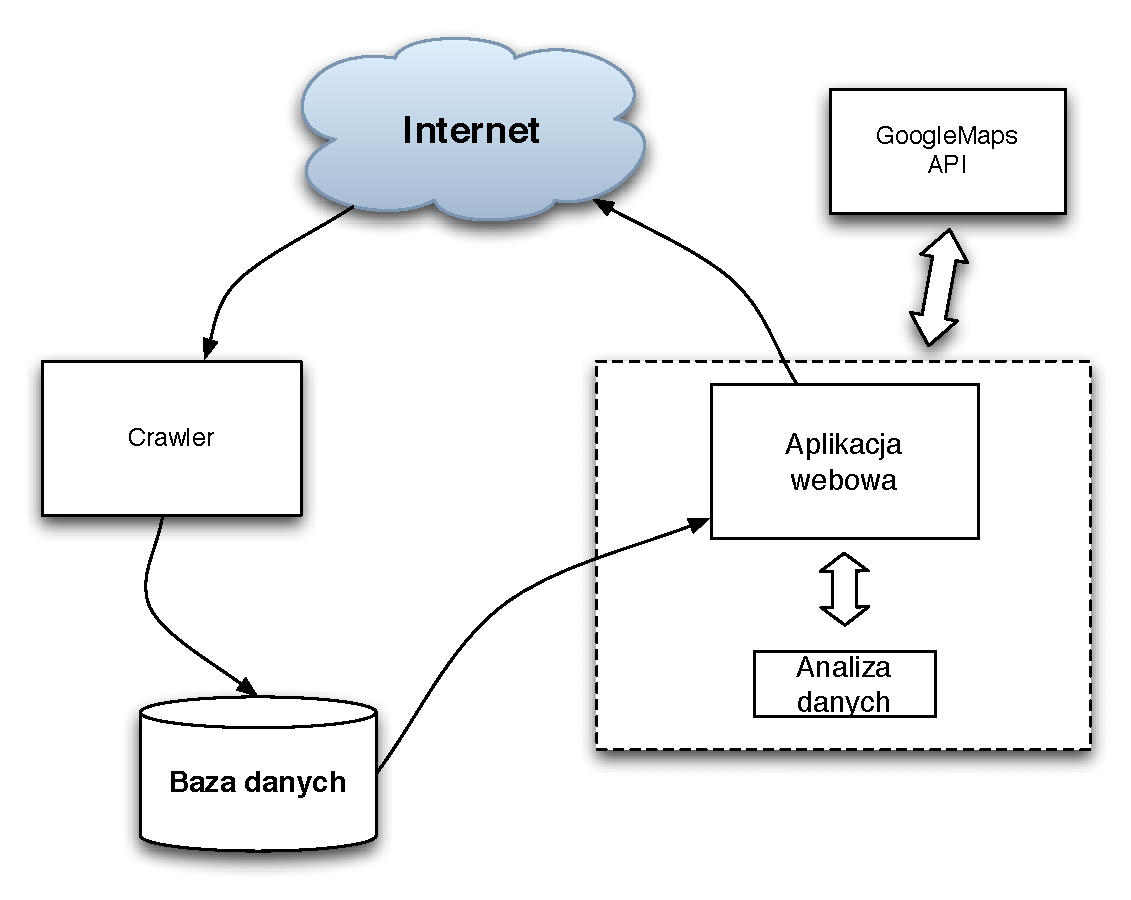
\includegraphics[width=35em]{images/data_flow_diagram.pdf}

\subsection{Entity Relationship Diagram}
Do momentu ustabilizowania bazy danych Oracle na serwerze AGH będziemy starali
się pracować na dostępnych za darmo silnikach typu Oracle Express (XE)
  postawionych na lokalnych maszynach, z uwzględnieniem możliwości
  przystosowania na nich aplikacji sprawnej w pełnej wersji Oracle. Wstępnie
  przewidujemy taki model istotnych danych:

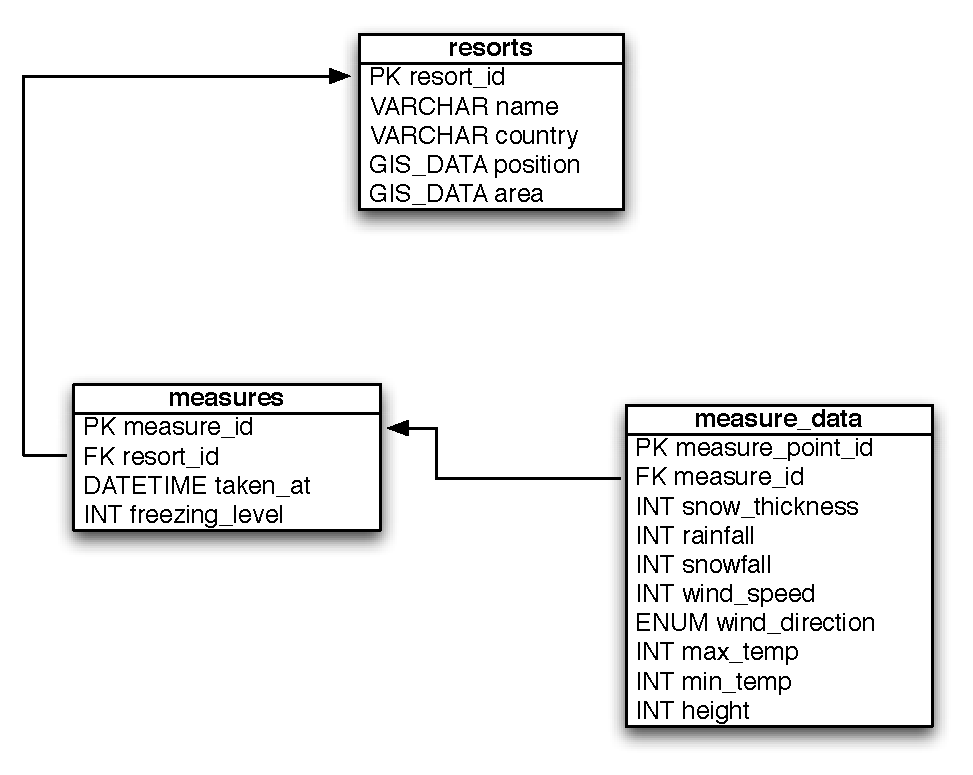
\includegraphics[width=35em]{images/erd_diagram.pdf}

\section{Aplikacja Django}
\subsection{Modele}
Zdefiniowane w aplikacji modele to:
\begin{description}
\item[WorldBorders] odpowiada za przechowywanie granic państw. Pola modelu:
  \begin{description}
  \item[name] nazwa państwa
  \item[lat] szerokość geograficzna
  \item[lon] długość geograficzna
  \item[mpoly] typ \emph{SDO\_GEOMETRY} przechowywujący \emph{MultiPolygon} który
    definiuje granice państwa
  \end{description}
\item[Resorts] przechowuje ośrodki dla których posiadamy dane pogodowe. Pola:
  \begin{description}
    \item[name] nazwa miasta
    \item[position] dwuwymiarowa geometria \emph{Point} przechowywująca długość i
      szerokość geograficzną miasta
  \end{description}
\item[Measures]
  \begin{description}
  \end{description}
\end{description}

\subsection{SQL}
\subsubsection{Stworzenie tabel}
Kluczowy dla projektu jest oczywiście typ \emph{SDO\_GEOMETRY} który umożliwia wykonywanie
specyficznych zapytań geograficznych. Reszta pól to dodatkowe informacje na temat państwa/miasta.
\begin{verbatim}
CREATE TABLE "WORLD_WORLDBORDERS" (
    "ID" NUMBER(11) NOT NULL PRIMARY KEY,
    "NAME" NVARCHAR2(50) NULL,
    "LAT" DOUBLE PRECISION NOT NULL,
    "LON" DOUBLE PRECISION NOT NULL,
    "MPOLY" MDSYS.SDO_GEOMETRY NOT NULL
);
\end{verbatim}

\begin{verbatim}
CREATE TABLE "WORLD_RESORTS" (
    "ID" NUMBER(11) NOT NULL PRIMARY KEY,
    "NAME" NVARCHAR2(50) NULL,
    "POSITION" MDSYS.SDO_GEOMETRY NOT NULL
);
\end{verbatim}

Tabela pomiarów posiada dodatkowo klucz obcy do ośrodków aby pomiar można było zaklasyfikować do
danego ośrodka.
\begin{verbatim}
CREATE TABLE "WORLD_MEASURES" (
    "ID" NUMBER(11) NOT NULL PRIMARY KEY,
    "RESORT_ID" NUMBER(11) NOT NULL REFERENCES "WORLD_RESORTS" ("ID")
         DEFERRABLE INITIALLY DEFERRED,
    "TEMP" NUMBER(11) NOT NULL,
    "TAKEN_AT" DATE NOT NULL
);
\end{verbatim}

\paragraph{Ustawienia metryki}
Aby Oracle wiedział, jak wygląda metryka, należy poinformować go ustalając odpowiednie wartości graniczne
oraz dokładność dla kolumn Spatial. W tym wypadku informujemy, że kolumna \emph{MPOLY} tabeli
\emph{WORLD\_WORLDBORDERS} posiada zakres długości od -180 do 180 oraz szerokości od -90 do 90 z dokładnością
co 0.05.

\begin{verbatim}
INSERT INTO USER_SDO_GEOM_METADATA
   ("TABLE_NAME", "COLUMN_NAME", "DIMINFO", "SRID")
   VALUES (
    'world_worldborders',
    'mpoly',
    MDSYS.SDO_DIM_ARRAY(
      MDSYS.SDO_DIM_ELEMENT('LONG', -180.0, 180.0, 0.05),
      MDSYS.SDO_DIM_ELEMENT('LAT', -90.0, 90.0, 0.05)
    ),
    4326
  );
\end{verbatim}

\paragraph{Indeksy}
Aby zapytania mogły funkcjonować należy stworzyć indeksy na kolumnach spatial. Służy do tego celu polecenie
\begin{verbatim}
CREATE INDEX "WORLD_RESORTS_POSITION_ID"
ON "WORLD_RESORTS"("POSITION")
INDEXTYPE IS MDSYS.SPATIAL_INDEX;
\end{verbatim}

\paragraph{Sekwencje}
Warto wspomnieć, że tabele mają klucze główne liczbowe i aby nie przejmować się ich numerowaniem
stworzyć należy sekwencje. Do tego celu użyliśmy:
\texttt{CREATE SEQUENCE WORLD\_WORLDBORDERS\_SQ}
i analogiczne dla pozostałych tabel.

\subsubsection{Spatial queries}
\paragraph{Ośrodki w pobliżu danego ośrodka}
\begin{verbatim}
SELECT "WORLD_RESORTS"."ID", "WORLD_RESORTS"."NAME",
       SDO_UTIL.TO_WKTGEOMETRY("WORLD_RESORTS"."POSITION")
FROM "WORLD_RESORTS"
WHERE
    (SDO_WITHIN_DISTANCE("WORLD_RESORTS"."POSITION",
        SDO_GEOMETRY(POINT (10.7498000000000005 46.9629699999999985), 4326),
        \'distance=20000.0\') = \'TRUE\'
    AND NOT ("WORLD_RESORTS"."ID" = 832))
\end{verbatim}
\emph{SDO\_WITHIN\_DISTANCE} to funkcja sprawdzająca czy geometria z pierwszego argumentu znajduje się w pewnej
odległości od geometrii drugiego. Jak widać drugą geometrię tworzymy przedstawiając dane geograficzne ośrodka
w postaci Well-Known Text: \texttt{POINT(10.749, 46.962)} pierwsza jest natomiast do tej postaci konwertowana
przez funkcję \emph{TO\_WKTGEOMETRY}. Trzeci argument to odległość jako liczba metrów. Cała
funkcja zwraca true gdy warunek spełniony.

\paragraph{Państwo, w którym znajduje się ośrodek}
\begin{verbatim}
SELECT "WORLD_WORLDBORDERS"."ID", "WORLD_WORLDBORDERS"."NAME",
       "WORLD_WORLDBORDERS"."LAT", "WORLD_WORLDBORDERS"."LON",
       SDO_UTIL.TO_WKTGEOMETRY("WORLD_WORLDBORDERS"."MPOLY")
FROM "WORLD_WORLDBORDERS"
WHERE SDO_CONTAINS("WORLD_WORLDBORDERS"."MPOLY",
    SDO_GEOMETRY(POINT (10.7498000000000005 46.9629699999999985), 4326)) = \'TRUE\'
\end{verbatim}
W tym wypadku używamy funkcji \emph{SDO\_CONTAINS} która zwraca prawdę, gdy druga gemoetria całkowicie zawiera pierwszą.
W naszym przypadku pierwszą geometrią jest wielobok przedstawiający granice państwa w tabeli państw natomiast druga to
punkt reprezentujący ośrodek. W ten sposób zwracamy wszystkie państwa których granice obejmująten punkt (w większości
przypadków będzie to jeden rekord).

\section{Crawler}
Crawler jest napisany w języku Ruby i służy do pobierania danych ze strony
\\\url{http://www.snow-forecast.com}.
Docelowo będzie to prosty skrypt oparty o metodologię \emph{Extract--Transform--Load}. W tej chwili zaimplementowana
jest część \emph{Extract}:
\begin{itemize}
\item uruchamiamy skrypt z parametrem adresu strony (w zasadzie chodzi o wybrany szczyt)
\item skrypt analizuje stronę za pomocą parsera HTML+XML Nokogiri
\item dane zapisywane są w prostej postaci w tablicy
\item skrypt znajduje link do danych z poprzedniego okresu, odwiedza go i powtarza proces
\end{itemize}

Dane są zapisywane w tej chwili w bardzo prostym formacie, część \emph{Transform} będzie odpowiedzialna
za ich konwersję do formatu odpowiedniego dla bazy danych

\section{Źródła}
Wszelkie źródła dostępne są do pobrania przez repozytorium Git pod adresem
\\
\url{http://github.com/michalbugno/projekt-oszdb/}

\end{document}
